\documentclass[a4j]{jarticle}
\usepackage{graphicx}

\title{コンパイラ実験 期末レポート}

\author{氏名: 木下直樹\\学籍番号: 09425521}

\date{出題日: 2015年4月13日\\提出日: 2015月7月27日\\締切日: 2015年7月27日}

\begin{document}
\maketitle

%%%%%%%%%%%%%%%%%%%%%%%%%%%%%%%
\section{実験の概要, 目的}
%%%%%%%%%%%%%%%%%%%%%%%%%%%%%%%
グループで定義した文法によるプログラムをアセンブリ言語に変換するコンパイラを作成し, コンパイラの構造や基本的な概念を学習する. 
コンパイラの作成は次のような工程で実施した. 
\begin{itemize}
\item BNFによる文法定義
\item 字句解析
\item 演算子順位構文解析
\item 再帰下降型構文解析
\item コード生成
\end{itemize}
作成したコンパイラで指定された最終課題と同じ動作をするアセンブリコードを生成する. 

また, コンパイラのソースプログラム, 課題1-4は以下のディレクトリに保存する.
\begin{verbatim}
/home/users/ecs/09425521/3zen
\end{verbatim}

%%%%%%%%%%%%%%%%%%%%%%%%%%%%%%%%%%%%%%%%%%%
\section{言語定義}
%%%%%%%%%%%%%%%%%%%%%%%%%%%%%%%%%%%%%%%%%%%
コンパイラの言語の定義はBNFで記述し, 文法は文脈自由文法とする. 複数の解釈が可能なあいまいな文法にならないようにする. 
言語定義とこの言語で受理される最終課題に対するプログラムコードをレポート末尾の付録に示す.

定義した言語には以下の基本機能を可能とするようにした.
\begin{itemize}
\item 変数への代入
\item 算術式の計算
\item 条件分岐
\item ループ
\item 配列
\end{itemize}

%%%%%%%%%%%%%%%%%%%%%%%%%%%%%%%%%%%%%%%%%%%
\section{字句解析}
%%%%%%%%%%%%%%%%%%%%%%%%%%%%%%%%%%%%%%%%%%%
この解析部では, 読み込んだプログラムコードの字句を解析する. 
解析部を以下の手順で作成する. 

\begin{enumerate}
\item 定義した文法中にでる字句の種類を整理する
\item 字句がどの状態にいるかを判断する定義を決め状態遷移図を作成する. 状態遷移図はレポート末尾の付録に示す. 
\item 作成した状態遷移図を表に書き換え, それが受理されるプログラムコードを書く. 
\end{enumerate}

分類するそれぞれの字句の名前はTokenTypeという型でdefine.hで定義し, 以上の手順で作成したプログラムで識別した字句にそのTokenTypeをリターンさせ, その字句が何者であるかを以降の作業で判断できるようにする. 
また, 分類するタイプに当てはまらない特定の文字列(define, while, forなど)はTokenType識別子の振るいに落ちた字句からさらに文字列の並びを調べ, 当てはまるものは予約語として追加定義したTokenTypeをリターンさせる. 


%%%%%%%%%%%%%%%%%%%%%%%%%%%%%%%%%%%%%%%%%%%%%%%%%%
\section{演算順位構文解析}
%%%%%%%%%%%%%%%%%%%%%%%%%%%%%%%%%%%%%%%%%%%%%%%%%%
この解析部では読み込むコード中の算術式を解析する. 
解析した算術式は数(または変数)と演算子をそれぞれ一つのtokenとして解析され, 定義した演算順位に従って木構造に変換される. 

変換した木の型Nodeは次の様にdefine.hで定義する. 

\begin{verbatim}
typedef struct node {
  TokenSt *token;              
  struct node *left;
  struct node *right;
  struct node *arg[TOKENMAX];
}Node;
\end{verbatim}

例えば, 1$+$2 を解析すると node に$+$ が格納され, node-$>$left, node-$>$right にそれぞれ 1, 2 が格納される. 
演算子が1つ以上登場する算術式ではこのようにトップノードに演算子, それにぶら下がる形で演算される値が格納されるようになり, 演算順位の高い計算は葉に近いnodeに格納される. 




%%%%%%%%%%%%%%%%%%%%%%%%%%%%%%%%%%%%%%%%%%%%%%%%%%
\section{再帰下降型構文解析}
%%%%%%%%%%%%%%%%%%%%%%%%%%%%%%%%%%%%%%%%%%%%%%%%%%
再帰下降型構文解析では, プログラムの頭から下向きに全体を解析する解析部を作成する. 
言語の定義通りに書かれないとエラーを起こすようなプログラムを記述していけばいいため, 定義をそのままプログラムにすればよいが, この解析部を作る前に文法定義で注意すべき点が二つある. 
後戻り(back tracking)と左再帰性(left-recursion)である. 

次のような文法定義では後戻りが発生する.
\begin{verbatim}
S ::= aBd
B ::= b | bc 
\end{verbatim}
この文法で文字列abcdを通すとBをbと解釈すると次のcで文法に合わないことになる. 
そのためBをbcと解釈し直すことになる. この解釈をやり直す工程を後戻りという. 
後戻りが発生する文法になっている箇所は文法自体は変更せず, 共通部分は分岐の前に処理を前倒しする くくりだし と呼ばれる処理をする.

また, 次のような文法は左再帰性を持ち, これは文法定義を変更する必要がある.
\begin{verbatim}
[左再帰] <文集合> ::= <文集合><文> | <文>
[変更後]  <文集合> ::= <文><文集合> | <文>
\end{verbatim}
上記のように構文の終わりで再帰するような文法に変更する. 

%%%%%%%%%%%%%%%%%%%%%%%%%%%%%%%%%%%%%%%%%%%%%%%%%%%
\section{コード生成}
%%%%%%%%%%%%%%%%%%%%%%%%%%%%%%%%%%%%%%%%%%%%%%%%%%%
構文解析の結果を元に, 目的のアセンブリコードを生成するプログラムを書く. 
算術式のアセンブリコードは演算構文解析のコードoparser.c中でスタックを用いた演算コードを生成し, それ以外のコードは再帰下降型構文解析のコードparse.c中の各解析処理で生成していく. 

%%%%%%%%%%%%
\subsection{メモリの扱い}
%%%%%%%%%%%%
本コンパイラでは局所変数のコード生成を作成していないため, 変数はすべて大域変数として扱う. 実際に格納するアドレスは0x10004000からで, 変数一つ(または配列の要素一つ)につき4バイトの領域を確保するため, 変数の数$×$4バイトの領域を確保させる. また, 変数の値は0が入れられた状態で宣言させる. 


%%%%%%%%
\subsection{レジスタの扱い}
%%%%%%%%%
プログラム中に飛び交う値がそれぞれの処理中に壊れないようにするために, その値を保持するレジスタの扱いを決めなければならない. 本プログラムでは以下の様にレジスタの扱いを取り決めた.
\begin{table}[htb]
  \begin{tabular}{lp{13cm}}
    算術式  & 計算対象に\$t0,\$t1レジスタを使い, 計算結果に\$v0を使用. 計算の瞬間にだけ使用.\\
    配列 & アドレスの計算に\$v0, \$t3, \$t4, \$t5レジスタを使用. 添字の値の解析に算術式を使い, その値は\$v0に入るため, そのまま\$v0を使用. 配列の先頭から目的の格納場所までのアドレス差の計算結果が\$t5に入れられる.\\
    条件判定 & 比較対象の値を\$v0, \$t8で扱い, その2数でslt命令をした結果を\$t3で預かる. \$v0, \$t8の値は算術式の結果であり, \$v0は算術式の結果をそのまま使用するため, \$v0の値が壊れないように先に\$t8に与える値を計算し, それを\$t8に移した後で\$v0の値の算術式を展開する.\\
    代入式 & 左辺の変数のアドレスを\$t2に保持し, 右辺の算術式の結果をそのアドレスへストアする. 右辺の解析が終わるまでの値保持のため, 算術式以外でなら使用可能. 
  \end{tabular}
\end{table}

%%%%%%%%%%%%
\subsection{記号表での管理}
%%%%%%%%%%%%
コンパイラ中で保持させたい変数や値などを管理するためにdefine.hで記号表を作成する. 

%%%%
\subsubsection{変数テーブル}
%%%%
変数の情報を管理するために以下のようなテーブルを作成した.
\begin{verbatim}
typedef struct {
  char name[TOKENMAX];
  int addr;
  int next;
  int subcount;       //添字[]の数
  int subamount[TOKENMAX];    //各添字の容量
  int addramount[TOKENMAX];   //アドレス計算で使用
}Vartable;            //変数
\end{verbatim}
\begin{itemize}
\item [name] 変数名を保持
\item [addr] 変数が格納されるアドレスを保持
\item [next] 次の変数が格納されるアドレスを保持
\item [subcount] 添字の数(配列でなければ0)
\item [subamount] 宣言された各添字の値
\item [addramount] 配列のアドレスを計算する際に使用
\end{itemize}


addramountにはsubamountを使って計算した結果を格納する. 以下がその計算部である. 
\\
\begin{verbatim}
  if(subcount){       // 配列のVartabel処理
    id[vi].subcount = subcount;
    x=subcount-1;
    id[vi].addramount[x]=4;
    for(x=subcount-1;x>=0;x--){
      id[vi].addramount[x-1] = id[vi].addramount[x] * id[vi].subamount[x];
    }
    id[vi].next = id[vi].addr + id[vi].addramount[0] * id[vi].subamount[0];
  }
\end{verbatim}

例えばa[5][6][7]が宣言されたときの処理は次の様な流れである.
\begin{verbatim}
addramount[2]=4  (配列の最後は常に4)
addramount[1]= addramount[2]*7 (=28)
addramount[0]= addramount[1]*6 (=168)
\end{verbatim}

%%%
\subsubsection{ループテーブル}
%%%
while, forループのために以下のようなテーブルを作成した. 
\begin{verbatim}
typedef struct{
  int flag;       
  Node *node;
  char string[100];
  int forflag;
  Node *fornode;
  char forstring[100];
}Looptable;
\end{verbatim}

\begin{itemize}
\item [flag] 条件式の比較演算子番号
\item [node] 条件式の右辺
\item [string] 条件式の左辺の変数
\item [forflag] for第三式のパターン
\item [fornode] for第三式の左辺(第三式が代入式出会った場合のみ使用)
\item [forstring] for第三式で値を代入する変数
\end{itemize}

whileとforは同じテーブルを使用する. 


%%%%%%%%%%%%%%%%%%%%%%%%%
\section{最終課題の実行結果}
%%%%%%%%%%%%%%%%%%%%%%%%%

定義した言語定義で書いたコードの実行結果を説明する. 
生成するコードはresult.s, compresult.sに書き込まれる.
最終課題は1から4まで実行し, 結果はcompresult.sのコードを採用する.
また, 変数や配列を宣言した際初期値0が与えられることや, 変数resultがデータセグメントの先頭に宣言されるのは仕様である. 

%%%%%%%%%%%%
\subsection{最終課題1}
%%%%%%%%%%%%

最終課題1は1から10までの数の和を計算するプログラムである. これを実行するためには変数, 代入式, ループ文, 算術式のコード生成が必要である. 

ループ文にforを採用した際の実行結果は次の様になった.
\begin{verbatim}
395 instructions

0x10004008 (268451848) = 0x00000037 (55)
\end{verbatim}
sumを格納したアドレス0x10004008のメモリに実行結果の55が格納されており, 実行ステップ数は413である. 
コンパイルしたソース言語は以下である.
\begin{verbatim}
main(){
  define i;
  define sum;

  for(i=1;i<11;i++){
  sum = sum + i;
  }
}
\end{verbatim}

%%%%%%%%%%%%%%
\subsection{最終課題2}
%%%%%%%%%%%%%%

最終課題2は階乗の計算である. 最終課題1が通ればこの課題も通るはずである. 

実行した結果は次の様になった. 
\begin{verbatim}
224 instructions

0x10004008 (268451848) = 0x00000078 (120)
\end{verbatim}
factを格納したアドレス0x10004008のメモリに実行結果の120が格納されており, 実行ステップ数は226である.
コンパイルしたソース言語は以下である.
\begin{verbatim}
main(){
  define i;
  define fact;

  fact = 1;
  for(i=1;i<6;i++){
    fact = fact * i;
  }
}
\end{verbatim}

%%%%%%%%%%%%%%
\subsection{最終課題3}
%%%%%%%%%%%%%%

最終課題3はエラトステネスと呼ばれる素数を調べるアルゴリズムである. 具体的には, すべての配列の要素に初期値1を与え, 素数でないものに随時0を代入するという処理を実行する. この課題に対応するためには, 2重ループと1次元以上の配列を使ったコードを受理できるコード生成を実現しなければならない. 

実行した結果は以下の様になった.

\begin{verbatim}
372779 instructions

0x10004000 (268451840) = 0x00000000 (0)
0x10004004 (268451844) = 0x000003e8 (1000)
0x10004008 (268451848) = 0x000001f5 (501)
0x1000400c (268451852) = 0x00000003 (3)
0x10004010 (268451856) = 0x00000000 (0)
0x10004014 (268451860) = 0x00000001 (1)
0x10004018 (268451864) = 0x00000001 (1)
0x1000401c (268451868) = 0x00000001 (1)
0x10004020 (268451872) = 0x00000000 (0)
0x10004024 (268451876) = 0x00000001 (1)
0x10004028 (268451880) = 0x00000000 (0)
0x1000402c (268451884) = 0x00000001 (1)
0x10004030 (268451888) = 0x00000000 (0)
0x10004034 (268451892) = 0x00000000 (0)
0x10004038 (268451896) = 0x00000000 (0)
0x1000403c (268451900) = 0x00000001 (1)
...
\end{verbatim}

配列の先頭アドレスは0x10004010であり, 実行ステップ数は379851である. 
コンパイルしたソースコードは以下である. 

\begin{verbatim}
main(){
  define N;
  define l;
  define m;
  define a[1001];
  N = 1000;

  for(l=1; l<=N; l++){ a[l] = 1;}

  for(l=2; l<=N/2; l++){
    for(m=2; m<=N/l; m++){
    a[l*m] = 0;
    }
  }
}
\end{verbatim}

%%%%%%%%%%%%%%%%%%%
\subsection{最終課題4}
%%%%%%%%%%%%%%%%%%%

最終課題4は2行2列の行列積の計算を行っている. これを実行するためには2次元配列のコード生成に対応しなければならない. 

実行した結果は以下の様になった. 

\begin{verbatim}
1319 instructions

0x10004024 (268451876) = 0x00000013 (19)
0x10004028 (268451880) = 0x00000016 (22)
0x1000402c (268451884) = 0x0000002b (43)
0x10004030 (268451888) = 0x00000032 (50)
\end{verbatim}
行列積の計算結果を格納する配列の先頭アドレスは0x10004024であり, 実行ステップ数は379851である. 

コンパイルしたソースコードは以下である. 

\begin{verbatim}
main(){
  define matrix1[2][2];
  define matrix2[2][2];
  define matrix3[2][2];

  define i;
  define l;
  define k;

  matrix1[0][0] = 1;
  matrix1[0][1] = 2;
  matrix1[1][0] = 3;
  matrix1[1][1] = 4;

  matrix2[0][0] = 5;
  matrix2[0][1] = 6;
  matrix2[1][0] = 7;
  matrix2[1][1] = 8;

  for(i=0;i<2;i++){
    for(l=0;l<2;l++){
      for(k=0;k<2;k++){
	matrix3[i][l] = matrix3[i][l] + matrix1[i][k] * matrix2[k][l];
      }
    }
  }
}
\end{verbatim}

%%%%%%%%%%%%%%%%%%%%%%%%%%
\section{考察}
%%%%%%%%%%%%%%%%%%%%%%%%%%

%%%%%%%%%%%%%%
\subsection{ループ文の実装}
%%%%%%%%%%%%%%

ループ文は開始前に条件判定し, 偽ならループ終了にジャンプし, 真ならジャンプせずにループ処理へ入る. ループ終了の直前では再度条件判定をし, 真ならループ開始ラベルへジャンプし, 偽ならジャンプせずにループ終了ラベルに落ちる. 保持しておきたいものをテーブルに格納することでループの終わりでの出力が可能になる. 

ループ文は条件判定を入れるタイミングは一つではないが, ループ前に条件判定をして偽ならループ終了ラベルへジャンプし, 真ならそのままループへ入る. そしてループ終了ラベルの手前で再度条件判定コードを設置し, 真ならループ開始ラベルへジャンプし, 偽ならそのままループ終了ラベルへ入る. 
この処理方式にすると命令数を減らすことができる. 

実際にループ開始直後に条件判定式を入れるだけのプログラムとの最終課題1での実行結果を比べた. 

\begin{itemize}
\item 条件判定部をループ開始直後に入れる場合\\
415 instructions
\item 条件判定部をループ開始前, ループ終了直前に入れる場合\\
395 instructions
\end{itemize}
実際に命令数が減っていることがわかる. 

%%%%%%%%%%%%%%%
\subsection{多次元配列の実装}
%%%%%%%%%%%%%%%
最終課題4の実行のために多次元配列を実装しなければならない. 
多次元配列の実装とは, 指定の配列要素のアドレスを算出する機能を持たせることである. 
アドレスを算出することができれば他の処理は配列でない変数と同じ振る舞いをすればよい. 

代入式等で配列のアドレスを算出するためにはその配列の宣言された添字と実際に計算で使用する配列要素の添字を使ってアドレスを算出すればよい. 
その計算を容易にするためにVartableに追加したsubcount, subamount, addramount をうまく計算に用いる. 

配列aの要素a[x][y][z](x,y,zは任意の整数)のアドレスを求めるときは以下の様に計算する.
\begin{verbatim}
addr=0;
addr=addr+addramount[0]*x;
addr=addr+addramount[1]*y;
addr=addr+addramount[2]*z;
\end{verbatim}
これをアセンブリ言語で出力し, 得られた値を配列の先頭アドレス(変数テーブルのaddr)を保持しているレジスタに加算するコードを出力すればよい. その後のロード等の命令は配列でない時と同じ仕様にする. 

%%%%%%%%%%%%%
\subsection{余分なコードの消去}
%%%%%%%%%%%%%

このコンパイラはコード生成の特性上余分なコードが発生する. 以下のようなコードが発生するため, それぞれコードを消去する.

\begin{enumerate}
\item sw \$v0, 0(\$t2) だけを出力
\begin{verbatim}
	addi $sp,$sp,-4
	sw $v0,0($sp)
	sw $v0, 0($t2)    #変数の値を更新
	addi $sp, $sp, 4
\end{verbatim}
\item add \$t8, \$v0, \$zero だけを出力
\begin{verbatim}
	addi $sp,$sp,-4
	sw $v0,0($sp)
	add $t8, $v0, $zero    #変数の値を更新
	addi $sp, $sp, 4
\end{verbatim}
\item 全行消去
\begin{verbatim}
	addi $sp,$sp,-4
	sw $v0,0($sp)
	addi $sp, $sp, 4
\end{verbatim}
\end{enumerate}

コードの消去を実装するのはmain.cで行う. 以下の様に出力ファイルresult.sを再度リードファイルとして読み込み, compresult.sに変更コードを出力する.
\begin{verbatim}
  while(fgets(data, 100, rfp) != NULL){
    if(strcmp(data,"\taddi $sp,$sp,-4\n") == 0){
      fgets(data[1], 100, rfp);
      if(strcmp(data[1], "\tsw $v0,0($sp)\n") == 0){
	fgets(data[2], 100, rfp);
	if(strcmp(data[2], "\tsw $v0, 0($t2)    #変数の値を更新\n") ==0 ||
	   strcmp(data[2], "\tadd $t8, $v0, $zero\n") == 0){
	  fgets(data[3], 100, rfp);
	  if(strcmp(data[3], "\taddi $sp, $sp, 4\n") == 0){
	    fprintf(cfp,data[2]);
	  }else{
	    fprintf(cfp,data);
	    fprintf(cfp,data[1]);
	    fprintf(cfp,data[2]);
	    fprintf(cfp,data[3]);
	  }
	}else if(strcmp(data[2], "\taddi $sp, $sp, 4\n") == 0){
	}else{
	  fprintf(cfp,data);
	  fprintf(cfp,data[1]);
	  fprintf(cfp,data[2]);
	}
      }else{
	fprintf(cfp,data);
	fprintf(cfp,data[1]);
      }
    }else{
      fprintf(cfp,data);
    }
  }
\end{verbatim}

最終課題3で出力結果を比較した結果以下の様になり, 命令数が1割近く減っているのがわかる.

\begin{itemize}
\item result.s\\
409202 instructions
\item compresult.s\\
372779 instructions
\end{itemize} 

%%%%%%%%%%%%%%%%%%%%%%%%%%
\section{付録}
%%%%%%%%%%%%%%%%%%%%%%%%%%

%%%%%%%%%%%%%
\subsection{言語定義}
%%%%%%%%%%%%%
\begin{verbatim}
<プログラム> ::= <変数宣言部> <関数群> | <関数群>
<変数宣言部> ::= <宣言文> <変数宣言部> | <宣言文>
<宣言文> ::= define <識別子>; | define <宣言配列>;
<宣言配列> ::= <識別子><定数添字列>
<定数添字列> ::= [数] | [数]<定数添字列>
<関数群> ::= <関数><関数群> | <関数>
<文集合> ::= <文> <文集合> | <文>
<文> ::= <代入文> | <ループ文> | <条件分岐文> | <関数文> 
<関数文> ::= <識別子>(<引数列>); | <識別子>();    /* 文集合から呼び出し */
<関数> ::= <識別子>(<仮引数列>){<変数宣言部><文集合>} | <識別子>(){<変数宣言部><文集合>}
<仮引数列>::=<仮引数><仮引数列>
<仮引数>::=<識別子> | <識別子>[]
<引数列> ::= <引数>, <引数列> | <引数>
<引数> ::= <算術式>
<代入文> ::= <識別子> = <算術式>; | <識別子><増減演算子>; | <配列> = <算術式>; | <配列><増減演算子>
<代入式> ::= <識別子> = <算術式> | <増減変数> | <配列> = <算術式>
<算術式> ::= <算術式> <加減演算子> <項> | <項> 
<項> ::= <項> <乗除演算子> <因子> | <因子>
<因子> ::= <変数> | (<算術式>) | <配列>
<加減演算子> ::= + | -
<乗除演算子> ::= * | /
<増減演算子> ::= ++ | --
<変数> ::= <識別子> | <数>
<増減変数> ::= <識別子><増減演算子> | <増減演算子><識別子> | <配列><増減演算子> | <増減演算子><配列>
<ループ文> ::= while(<条件式>){<文集合>} | for(<識別子> = <数>;<条件式>;<代入式>){<文集合>)}| for(<配列> = <数>;<条件式>;<代入式>){<文集合>)}
<配列> ::= <識別子><添字列> 
<添字列> ::= [<変数>] | [<変数>]<添字列> | [<配列>]<添字列>
<条件分岐文> ::= if(<条件式>){<文集合>} | if(<条件式>){<文集合>}else{<文集合>}
<条件式> ::= <識別子><比較演算子><算術式> | <配列><比較演算子><算術式>
<比較演算子> ::= == | '<' | '>' | != | '<'= | '>'=
<識別子> ::= <英字> <英数字列> | <英字>
<英数字列> ::= <英数字> <英数字列> | <英数字>
<英数字> ::= <英字> | <数>
<数> ::= <自然数字><準数> | <数字>
<準数> ::= <数字><準数> | <数字>
<自然数字> ::= 1|2|3|4|5|6|7|8|9
<英字> ::= a|b|c|d|e|f|g|h|i|j|k|l|m|n|o|p|q|r|s|t|u|v|w|x|y|z|
       A|B|C|D|E|F|G|H|I|J|K|L|M|N|O|P|Q|R|S|T|U|V|W|X|Y|Z
<数字> ::= 0|<自然数字>
\end{verbatim}

%%%%%%%%%%%%
\subsection{プログラム例}
%%%%%%%%%%%%
以下に定義した文法に沿ったプログラム例を添付する. 
作成したコンパイラではエラーなく読み込むことができるものの, 関数呼出と局所変数のコード生成部が完了していないため, 生成したプログラムコードを正常に実行することはできない. 
\begin{verbatim}
define x;
define y;

main(){
  define l;
  define m;
  define n;

  x=0;

  while(l<10){
    x=x+1;
    l++;
  }

  for(m=10; m!=0; m--){
    y=y+2;
  }

  mult(x,y);

  if(result == 200){
    x=1;
  }else{
    x=0;
  }
}

mult(a, b){
  result = a*b;
}
\end{verbatim}

%%%%%%%%%%%%
\subsection{遷移表}
%%%%%%%%%%%%

\begin{table}[htb]
\scalebox{0.75}{
\begin{tabular}{|l|l|l|l|l|l|l|l|l|l|l|l|l|l|l|l}
 
\hline
& 0 & 1$-$9 & 英字 & $<$,$>$ & $=$ & $!$ & ;,(,),\{,\},[,]& $+$ & $-$ & $*$,$/$\\
\hline
初期状態 &数&数&識別子&単一比較&単一比較&NOT&区切り&加算&減算&乗除演算子\\
\hline
数&数&数&終了状態&終了状態&終了状態&終了状態&終了状態&終了状態& 終了状態&終了状態  \\
\hline
識別子&識別子&識別子&識別子&終了状態&終了状態&終了状態&終了状態&終了状態&終了状態&終了状態\\
\hline
単一比較&終了状態&終了状態&終了状態&終了状態&二重比較&終了状態&終了状態&終了状態& 終了状態& 終了状態\\
\hline
二重比較&終了状態&終了状態&終了状態&終了状態&終了状態&終了状態&終了状態&終了状態& 終了状態& 終了状態\\
\hline
NOT&エラー&エラー&エラー&エラー&NOTEQ&エラー&エラー&エラー&エラー&エラー\\
\hline
NOTEQ&終了状態&終了状態&終了状態&終了状態&終了状態&終了状態&終了状態&終了状態& 終了状態& 終了状態\\
\hline
区切り&終了状態&終了状態&終了状態&終了状態&終了状態&終了状態&終了状態&終了状態& 終了状態& 終了状態\\
\hline
加算&終了状態&終了状態&終了状態&終了状態&終了状態&終了状態&終了状態&増減演算子& 終了状態& 終了状態\\
\hline
減算&終了状態&終了状態&終了状態&終了状態&終了状態&終了状態&終了状態&終了状態& 増減演算子& 終了状態\\
\hline
増減演算子&終了状態&終了状態&終了状態&終了状態&終了状態&終了状態&終了状態&終了状態& 終了状態& 終了状態\\
\hline
乗除演算子&終了状態&終了状態&終了状態&終了状態&終了状態&終了状態&終了状態&終了状態& 終了状態& 終了状態\\
\hline
\end{tabular}}
\caption{遷移表}
\label{tab:遷移表}
\end{table}


%%%%%%%%%%%%
\subsection{遷移図}
%%%%%%%%%%%%

\begin{table}[htb]
\begin{center}
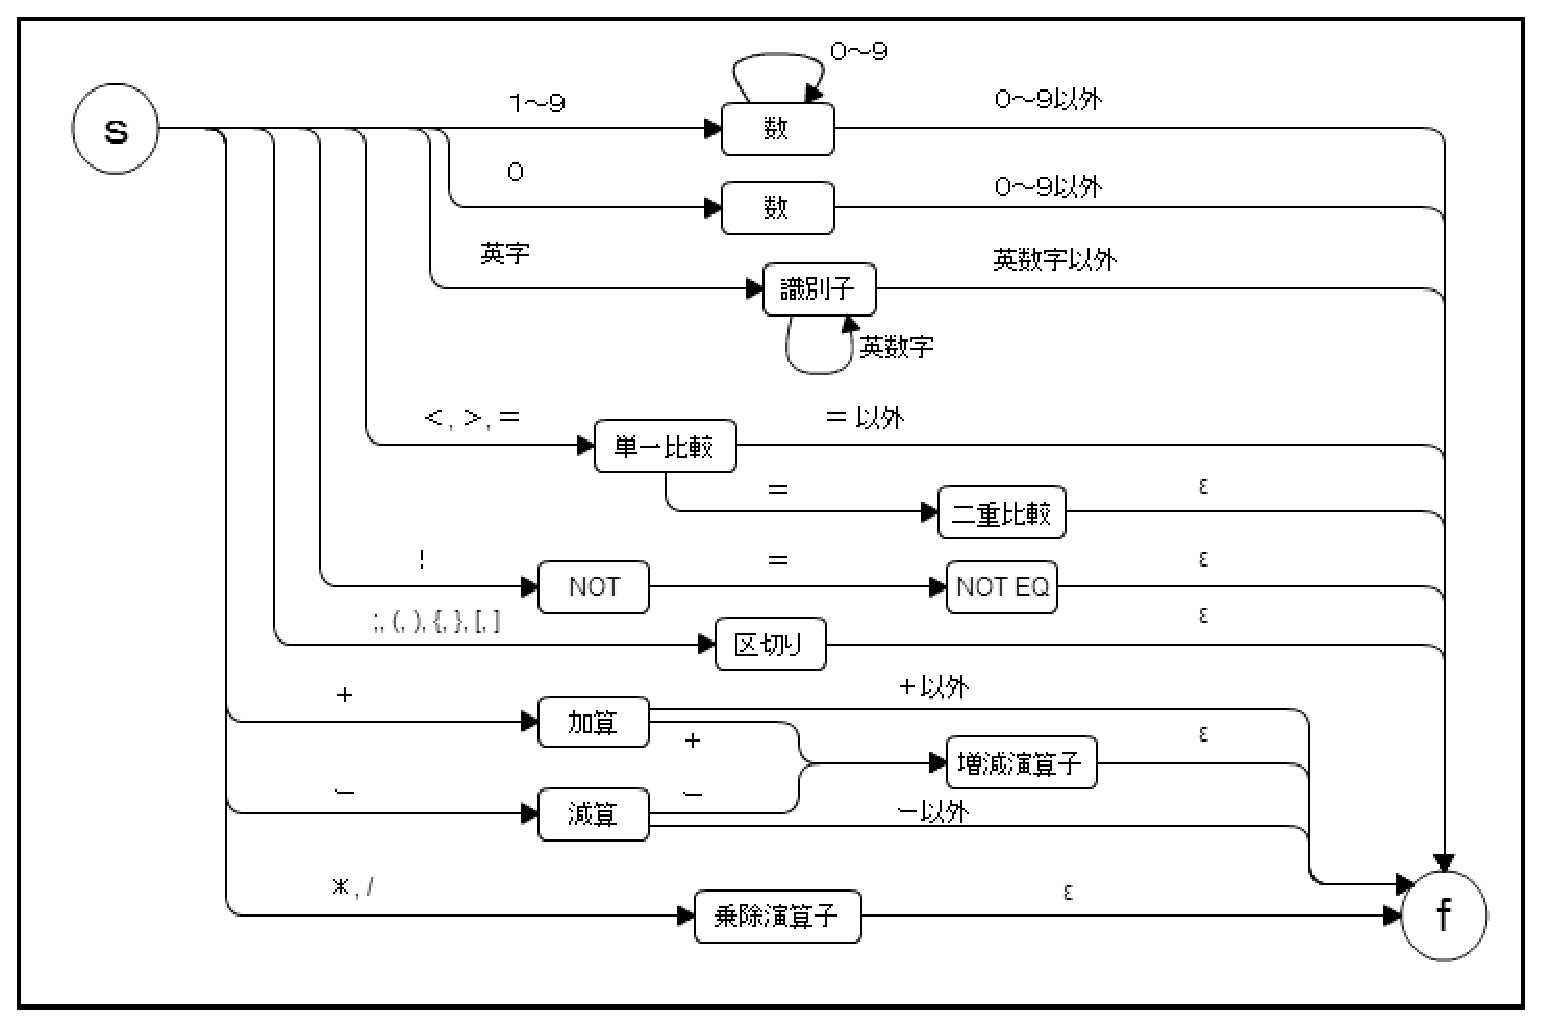
\includegraphics[scale=0.45]{senizu.eps}
\caption{遷移図}
\label{tab:遷移図}
\end{center}
\end{table}



\end{document}

































